%%!TEX ROOT = ../mainCZ.tex
% 
% 
% 
%
% Plošný povrchový odtok
%
%
%

\section{Bilanční rovnice} 

% 
Základním řešeným vztahem je aktuální bilance celkové zásoby
\begin{equation}
\acs{dS} = \acs{Itot} - \acs{Otot},
\label{eq:bilobecne}
\end{equation}
% 
% 
% 
% kde se aktuální změna  zásoby $S$ rovná rozdílu sumy aktuálních přítoků  \acs{Itot} a sumy aktuálních odtoků \acs{Otot}.
\begin{tabular}{rrl}
  kde \jj{dS}{,}
      \jj{Itot}{,}
      \jj{Otot}{.}
\end{tabular}


Podle složek povrchového odtoku a dalších procesů lze \acs{Itot} a \acs{Otot} v rovnici~(\ref{eq:bilobecne}) dále rozepsat na
$$
  \acs{Itot} = \acs{ES} + \acs{Oin},
$$
$$
  \acs{Otot} = \acs{Inf} + \acs{Oout},
$$
% 
% kde \acs{Oin} je přítok ze sousední výpočetní buňky (buněk) a \acs{Oout} je odtok z dané buňky. 
\begin{tabular}{rrl}
  kde \jj{Oin}{,}
      \jj{Oout}{,}
      \jj{ES}{,}      
      \jj{Inf}{.}
\end{tabular}


Bilanční rovnici v buňce $i$ v čase $t$ lze rozepsat jako:




\begin{equation} 
\frac{\mathrm{d}S}{\mathrm{d}t} = \acs{ES}_{i,t-1} + \sum_j^m \acs{Oin}_{j,t-1} - \acs{Inf}_{i,t-1} - \acs{Oout}_{i,t-1},
\label{eq:bilancnirceV}
\end{equation}
% 
% 
% 
% kde $m$ jsou buňky, odkud vtéká voda do buňky $i$. 
\begin{tabular}{rrl}
  kde & $m$ & jsou buňky, z nichž vtéká voda do buňky $i$. 
\end{tabular}


V aktuální verzi modelu \smod se $m$ řídí pomocí jednosměrného odtokového algoritmu \acs{D8}.
% se liší podle použitého odtokového algoritmu jednosměrného \acs{D8} nebo vícesměrného \acs{mfda} ({\it multi-flow direction algorithm}) \pozn{ citace}. 
Model \smod řeší časový krok explicitně, veličiny v čase $t-1$ na pravé straně rovnice (\ref{eq:bilancnirceV}) jsou při řešení času $t$ známé.
% Objem srážky \acs{ES} a infiltrované množství \acs{Inf} lze určit přímo při výpočtu časového kroku $t$. Přiteklé a odteklé množství vody \acs{Oin} a \acs{Oout} z časového kroku $t-1$ (což odpovídá explicitnímu řešení časové derivace). 




Při samotném řešení se v modelu \smod operuje s veličinami ve výškových jednotkách ($m$) a intenzitách ($m/s$). Pokud celou rovnici~(\ref{eq:bilancnirceV}) vydělíme velikostí buňky \acs{bunka} a vyjádříme časovou derivaci jako diferenci ($\frac{\mathrm{d}\acs{hsur}_{i,t}}{\mathrm{d}t} \approx \frac{\acs{hsur}_{i,t} - \acs{hsur}_{i,t-1}}{\acs{dT}}$), vypadá rovnice~(\ref{eq:bilancnirceV}) následovně:

%nejsou to náhodou objemové jednoty, které dělíme plochou

\begin{equation} 
\acs{hsur}_{i,t} = \acs{hsur}_{i,t-1} + \acs{dT}\left(\acs{es}_{i,t-1} + \sum_j^m \acs{oin}_{j,t-1} - \acs{inf}_{i,t-1} - \acs{oout}_{i,t-1}\right),
\label{eq:bilancnirce}
\end{equation}
% 
% 
% 
% 
% kde \acs{hsur} je výška hladiny na povrchu, \acs{es} je intenzita srářky, \acs{inf} je intenzita infiltrace, \acs{oin}(\acs{oout}) odteklá (přiteklá) výška za čas. 
\begin{tabular}{rrl}
  kde \jj{hsur}{,}
      \jj{es}{,}
      \jj{inf}{,}
      \jj{oin}{,}
      \jj{oout}{.}
\end{tabular}
% 
% 


V následujícím textu jsou popsány jednotlivé členy na pravé straně rovnice~(\ref{eq:bilancnirce}).


% 
% 
% 
% 
% 
% 
% Efektivní srážka \acs{ES}
% 
% 
% 
% 
% 
% 
% 
\subsection{Efektivní srážka \acs{es}} 

Srážka je příčinou celého erozního procesu. Vzhledem k tomu, že je \smod epizodní model zadává se srážka v podobě konkrétní nebo návrhové srážky, která začíná s prvním časovým krokem výpočtu. Model počítá s vlivem intercepce, která je definována pomocí potenciální intercepce \acs{PotI} jako výška zachycené vody. Míra zachycení v každém časovém kroku (\acs{dT}) výpočtu je definována  pomocí poměrné plochy listové \acs{Lai} (například \pozn{ citace}).

Označme množství srážky, které dopadá na povrch půdy i rostliny během \acs{dT} potenciální srážkou \acs{PS}. Část \acs{PS}, která zůstane  na povrchu rostliny během časovém kroku \acs{dT}, se dá vyjádřit jako násobek srážky \acs{PS} a \acs{Lai},
$$
\acs{PS}\ I_{LAI}.
$$
% 
Z tohoto vztahu vyplývá, že množství, které propadne povrchem listů, je 
$$
\acs{PS}(1 - I_{LAI}).
$$

Potenciální intercepce \acs{PotI} se začne plnit na začátku srážkové epizody. Po naplnění \acs{PotI} dopadá celá srážka na povrch půdy. Výsledná intenzita efektivní srážky v čase $t$ je pak určena jako

$$
   \acs{es}_t= 
    \begin{cases}
     \acs{PS}_t(1 - I_{LAI})\acs{dT},& \text{pokud} \sum_{\bar{t} = t_{init}}^{t} (\acs{PS}_{\bar{t}}\ I_{LAI}) <= \acs{PotI}\\
     \acs{PS}_t\acs{dT},             & \text{jinak}
   \end{cases}
$$


% $$
%  \acs{es}_t = MAX(0;\sum_{\bar{t} = t_{init}}^{t}\left(\acs{PS}_{\bar{t}}(1 - I_{LAI})\right)-\acs{PotI}))/\acs{dT},
% $$
% kde suma $\sum_{\bar{t} = t_{init}}^{t}$ vyjadřuje množství srážky které propadlo povrchem listů plodiny od počátečního času $t_{init}$ do času $t$.
\begin{tabular}{rrl}
  kde \jj{PS}{,}
      \jj{Lai}{,}
      \jj{PotI}{\ a}
      & $\sum_{\bar{t} = t_{init}}^{t} (\acs{PS}_{\bar{t}}\ I_{LAI}) $ & vyjadřuje množství srážky, které propadlo \\
      && povrchem listů plodiny od počátečního času $t_{init}$ do času $t$.
      \label{srazka}
\end{tabular}



% 
% 
% 
% 
% 
% 
% 
% 
% 
% 
\subsection{Intenzita infiltrace \acs{inf}}

V modelu je použita infiltrace podle Philipa \citep{philip1957} v~následujícím tvaru:
\begin{eqnarray} \label{eq:phillip}
\acs{inf} = \frac{1}{2}\acs{Sorb}t^{-1/2}+\acs{Ks}.
\end{eqnarray}
% 
% 
\begin{tabular}{rrl}
  kde \jj{inf}{,}
      \jj{Sorb}{\ a}
      \jj{Ks}{.}
\end{tabular}




Philipova infiltrační rovnice byla zvolena především z důvodu relativně malého počtu vstupních parametrů. Tato zjednodušená rovnice má dva členy: nasycenou hydraulickou vodivost \acs{Ks} a sorptivitu \acs{Sorb}. Autoři modelu si byli vědomi omezení použití Philipovy rovnice vyplývající z podmínek, za kterých byla odvozena.  Možné odchylky způsobené volbou této rovnice odpovídají odchylkám v heterogenitě půdy a rozptylu ostatních vstupních parametrů, na jejichž základě model pracuje. Čas $t$ ve vztahu~(\ref{eq:phillip}) je čas od začátku srážky, který by měl být v epizodním modelu totožný s počátečním časem výpočtu. Tato nezbytná podmínka by měla být brána v potaz při přípravě vstupních dat. 
% 
% 
% 
% 
% 
% 
% 
% 
% 
% 
% 
\section{Povrchový odtok  \acs{oin}, \acs{oout}} \label{sec:povrch_odtok}


V modelu jsou uvažovány dvě složky povrchového odtoku: \textbf{plošný povrchový odtok} a \textbf{soustředěný odtok v rýhách}. Soustředěný odtok v rýhách je ve \smod řešen explicitně. Vznik soustředěného odtoku je podmíněn překročením limitní rychlosti, resp. limitního tečného napětí (viz kapitola \ref{sec:soustredenyodtok}).

\subsection{Plošný povrchový odtok} \label{sec:plosny_odtok}

Rovnice plošného odtoku vychází ze zjednodušení Saint-Venantových (SV) rovnic použitím teorie kinematické vlny. Použití toho přístupu předpokládá mělké povrchové proudění po dlouhém plochém\footnote{Plochém ve smyslu ne příliš zakřiveném. Nejedná se tedy o hladký povrch.} povrchu. Za těchto podmínek lze u pohybové rovnice SV rovnic zanedbat lokální změny kinetické a potenciální energie a lokální zrychlení. Při tomto zjednodušení lze uvažovat povrchový tok jako ustálené proudění~\citep{miller1984basic}. Plošný povrchový odtok pak lze řešit pomocí obecného mocninného vztahu 
% 
% 
% 
\begin{equation}
  \acs{qsur} = \acs{a}\acs{hsur}^{\acs{b}},
  \label{eq:plos_prutok}
\end{equation}
% 
% 
% 
\begin{tabular}{rrl}
  kde \jj{qsur}{,}
      \jj{a}{\ a}
      \jj{b}{.}
\end{tabular}\\
Parametr \acs{a} je řešen podle vztahu:
$$
a = \acs{X}\acs{I}^{\acs{Y}},
$$
\begin{tabular}{rrl}
  kde \jj{X}{,}
      \jj{Y}{\ a}
      \jj{I}{.}
\end{tabular}

Parametry \acs{a} a \acs{b} respektive \acs{X} a \acs{Y} jsou odvozeny na základě měření \citep{Neumann15:232823}, jejich hodnoty pro různé půdní typy jsou ukázány v tabulce~\ref{tab:kriticke} v příloze~\ref{sec:priloha}. Z vyhodnocení vyplývá, že parametr \acs{b} je závislý pouze na půdním druhu. Parametr \acs{a} je závislý nejen na půdním druhu, ale také na sklonu svahu $I$. Pokud je  povrch půdy pokryt vegetací, je třeba provést korekci pomocí Manningova součinitele drsnosti pro povrchový odtok, který reprezentuje tření mezi tokem a vegetací. Parametr \acs{a} je pak definován jako
$$
  a = \frac{\acs{X}\acs{I}^{\acs{Y}}}{100\acs{n}},
$$
\begin{tabular}{rrl}
  kde \jj{n}{.}
\end{tabular}



Odteklá resp. přiteklá výška je pak dopočítána jako
$$
   \acs{oout} (resp.\ \acs{oin}) = \frac{\acs{effVrst}}{\acs{bunka}}\acs{qsur}
$$
%
% 
\begin{tabular}{rrl}
  kde \jj{effVrst}{\ a}
      \jj{bunka}{.}
\end{tabular}

Efektivní vrstevnice \acs {effVrst} je největší délka v buňce rastru kolmá na směr odtoku. Jedná se tedy o délku průmětu průtočné plochy na danou buňku.

% $$
% q_{sur} [m^{3}/s] = Ah_{sur}^{b} \Rightarrow \frac {1}{n} a h_{sur}^{X} i_{0}^{Y}
% $$


% 
% 
% 
% 
% 
% 
% 
% 
% 
% 
% 

\subsubsection{Odvozené veličiny}

Z vypočteného specifického průtoku, velikosti řešeného elementu a délky časového kroku lze dopočítat objem odtoku:
$$
  \acs{Vout} = \acs{dT}\ \acs{effVrst}\acs{qsur},
$$
% 
% 
% 
% 
\begin{tabular}{rrl}
  kde \jj{Vout}{.}
\end{tabular}


Pro posouzení erozního ohrožení a pro určení vzniku rýhy je v každé buňce vypočítávána rychlost proudění a tečné napětí. Za předpokladu, že se jedná a proudění vody o malé hloubce, lze rychlost proudění odvodit ze specifického průtoku a výšky hladiny:
% 
% 
% 
% 
% 
\begin{equation}
  \acs{vsur} =  \frac{\acs{qsur}}{\acs{hsur}},
  \label{eq:v}
\end{equation}
% 
% 
% 
\begin{tabular}{rrl}
  kde \jj{vsur}{.}
\end{tabular}
% 
Vztah pro výpočet tečného napětí je v modelu \smod definován podle \cite{Schwab1993} jako
% 
% 
% 
\begin{equation}
\acs{tausur} = \acs{ro} \acs{g} \acs{hsur} \acs{I}\acs{K},
 \label{eq:tau}
\end{equation}
% 
% 
% 
\begin{tabular}{rrl}
  kde \jj{tausur}{,}
      \jj{ro}{,}
      \jj{g}{,}
      \jj{I}{\ a}
      \jj{K}{.}
\end{tabular}

\subsubsection{Určení vzniku rýhy}\label{sec:vznikryhy}

Povrchový odtok způsobuje tření na povrchu půdy. Za určitých podmínek je soudržnost půdy nižší než tečné napětí proudící vody na jejím povrchu. Je několik způsobů jak tento moment určit \pozn{citace}. V modelu \smod jsou implementovány dva způsoby odvození: překročením kritického tečného napětí a překročením nevymílací rychlosti. Z obou odvození je určena kritická výška hladiny povrchového odtoku \acs{hcrit}  po jejímž překročení začne vznikat rýha. 


Při vzniku rýh dochází k velkému odnosu půdy, proto by umístění prvků protierozní ochrany mělo být navrhnuto tak, aby k vniku rýh docházelo co nejméně. Kritické hodnoty nevymílacích rychlostí a tečných napětí jsou pro jednotlivé půdní druhy převzaty z předchozích verzí modelu \citep{DyrovaE.1984, Neumann15:232823}. Hodnoty z obou zdrojů jsou ukázány v tabulce~\ref{tab:kriticke} v příloze~\ref{sec:priloha}.
V literatuře se setkáme i s odlišnými hodnotami. Například M. A. Velikanov stanovil kritickou nevymílací rychlost pro půdy 0.24 $m/s$  \citep{CabikJ.1963}, což je hodnota nižší, než kterou stanovila E. Dýrová. Při větších aplikacích modelu se doporučuje provést rekalibraci parametrů pro dané specifické území. 



Přepočet kritické nevymílací rychlost na kritickou výšku hladiny \acs{hcrit} je odvozen z rovnic (\ref{eq:plos_prutok}) a (\ref{eq:v}) jako
\begin{equation}
  \acs{hcrit}_{,v} = \frac{100\ \acs{n}\ \acs{vcrit}^{1/(\acs{b}-1)}}{\acs{a}},
  \label{eq:hcrit_v}
\end{equation}
\begin{tabular}{rrl}
  kde \jj{hcrit}{\ a}
      \jj{vcrit}{.} 
%   
\end{tabular}


Výpočet kritické výšky hladiny z tečného napětí je jednoduše odvozen z vzorce (\ref{eq:tau}) jako
\begin{equation}
  \acs{hcrit}_{,\tau} = \frac{\acs{taucrit}}{\acs{ro} \acs{g} \acs{I}},
  \label{eq:hcrit_tau}
\end{equation}
% 
\begin{tabular}{rrl}
  kde \jj{taucrit}{.} 
%   
\end{tabular}


Pro každou buňku výpočetní oblasti je spočítáno \acs{hcrit} pomocí obou odvození (\ref{eq:hcrit_v}) a (\ref{eq:hcrit_tau}). Podmínka v modelu následně vybere menší z hodnot
$$
  \acs{hcrit} = MIN(\acs{hcrit}_{,v},\acs{hcrit}_{,\tau}),
$$
která je pak pří výpočtu použita jako kritérium vzniku rýh. Kritická výška odvozená podle vztahu  (\ref{eq:hcrit_tau}) nebere v potaz parametry rovnice kinematické vlny a především pro malé hodnoty Manningova koeficientu \acs{n} (při řídkém nebo žádném vegetačním pokryvu) může být kritická hodnota \acs{hcrit} menší při použití rovnice (\ref{eq:hcrit_v}). Výběr menší hodnoty \acs{hcrit} by měl zamezit podhodnocení rizika vzniku rýhové eroze. 
 
Kritická nevymílací rychlost a kritické tečné napětí jsou vstupní parametry modelu. Návrh hodnot pro model \smod je ukázán v tabulce~\ref{tab:kriticke} v příloze~\ref{sec:priloha}. 



% 
% 
% 
% 
% 
% 
% 
% 
% 
% 
% 
\subsection{Soustředěný odtok v rýhách} \label{sec:soustredenyodtok}

Výpočet soustředěného odtoku v rýhách implementovaný v modelu SMODERP vychází z~několika předpokladů:
\begin{enumerate}
  \item Zavedením stejných zjednodušujících předpokladů výpočtu proudění jako v~případě výpočtu plošného povrchového odtoku (teorie kinematické vlny), lze řešit tok rýhou jako ustálené proudění.
  %Předpokladem je, že se tok ve všech časech a ve všech buňkách vždy dostane do ustáleného, tady že se vždy jedná o ustálené proudění. 
  Při ustáleném proudění se předpokládá sklon \pozn{nebo to byt sklon treci síly?} dna \acs{I} paralelní se sklonem hladiny vody v rýze a neměnná drsnost v celé délce buňky. Průtok v rýze je tedy vyjádřen pomocí Manningovy rovnice:
  \begin{equation}
    \acs{qrill} = \acs{vrill} \acs{A} = \acs{A} \frac{1}{\acs{n}} \acs{Rrill}^{2/3} \acs{I}^{1/2}  ,
    \label{eq:qrill}
  \end{equation}
  \begin{tabular}{rrl}
    kde \jj{qrill}{,}
        \jj{vrill}{,}
        \jj{A}{,}
        \jj{n}{\ a}
        \jj{Rrill}{.}
  \end{tabular}

  \item V každé buňce výpočetní oblasti může vzniknout pouze jedna přímá rýha bez ohledu na velikost buňky. 
  
  
  \item Soustředěný odtok vzniká v buňkách, kde dojde k překročení kritické výšky hladiny \acs{hcrit} (viz \ref{sec:vznikryhy}). Tato hodnota je určena pro každou buňku zvlášť na základě  hodnot kritického tečného napětí nebo kritické nevymílací rychlostí podle vzorců (\ref{eq:hcrit_v}) a (\ref{eq:hcrit_tau}).
  
  
  
  
  \item Objem vzniklé rýhy odpovídá nadkritickému objemu vody \acs{Vrill}, který vychází ze vztahu:
  $$
  \acs{Vrill}= \acs{Vtot} - \acs{Vcrit} = MAX(0;\acs{hsur} - \acs{hcrit}) \acs{bunka}
  $$
  \begin{tabular}{rrl}
    kde \jj{Vrill}{,}
        \jj{Vtot}{,}
        \jj{Vcrit}{\ a}
        \jj{hcrit}{.}
  \end{tabular}
  

  \item Tvar příčného profilu rýhy je reprezentován obdélníkem s pevným poměrem stran \acs{rratio}=výška/šířka rýhy. Velikost rýhy se zvětšuje pokud je nadkritické množství \acs{Vrill} větší než objem samotné rýhy, tak aby byl splněn předpoklad v předchozím bodě. Při zvětšovaná rýhy se tedy výška rýhy rovná výšce vodní hladiny v rýze (obrázek~\ref{fig:rill_plneni}). Pokud začne být nadkritické množství \acs{Vrill} menší než je objem rýhy a dochází k prázdnění rýhy,  zůstává velikost rýhy  konstantní a v rýze dochází pouze k poklesu hladiny (obrázek~\ref{fig:rill_prazdneni}). Tento mechanizmus ovlivňuje odtok pomocí hydraulického poloměru, který je u obdélníkového příčného profilu odvozen jako 
  $$ 
    \acs{Rrill} = \frac{\acs{A}}{\acs{O}} = \dfrac{\acs{hrill} \acs{brill}}{\acs{brill}+2\acs{hrill}} 
  $$
  \begin{tabular}{rrl}
    kde \jj{brill}{\ a}
        \jj{O}{.}
%         \jj{rratio}{.}
  \end{tabular}
  
  Při plnění nebo prázdnění se v tomto vztahu liší výpočet základny tohoto obdélníku. Pokud se rýha zvětšuje nebo je konstantní, určuje se šířka základny jako (obrázek~\ref{fig:rill_plneni})
  $$
    \acs{brill} = \dfrac{\acs{hcrit}}{\acs{rratio}} = \dfrac{\acs{yrill}}{\acs{rratio}},
  $$
  \begin{tabular}{rrl}
        \jj{rratio}{.}
  \end{tabular}
  
  Pokud se rýha prázdní je šířka rýhy odvozena jako (obrázek~\ref{fig:rill_prazdneni})
  $$
    \quad \acs{brill} = \dfrac{\acs{yrill}}{\acs{rratio}}.
  $$
  
  Jak je vidět na obrázku~\ref{fig:rill_prazdneni}, k plošnému povrchovému odtoku s výškou hladiny \acs{hcrit} dochází i na části buňky, kde se vytvořila rýha. Chyba vzniklá tímto předpokladem je považována za zanedbatelnou, protože plocha, kterou pokrývají rýhy, je zpravila malá proti ploše celého povodí. 
  
  

  \begin{figure}[t]
    \begin{subfigure}[b]{1.\linewidth}
      \centering
      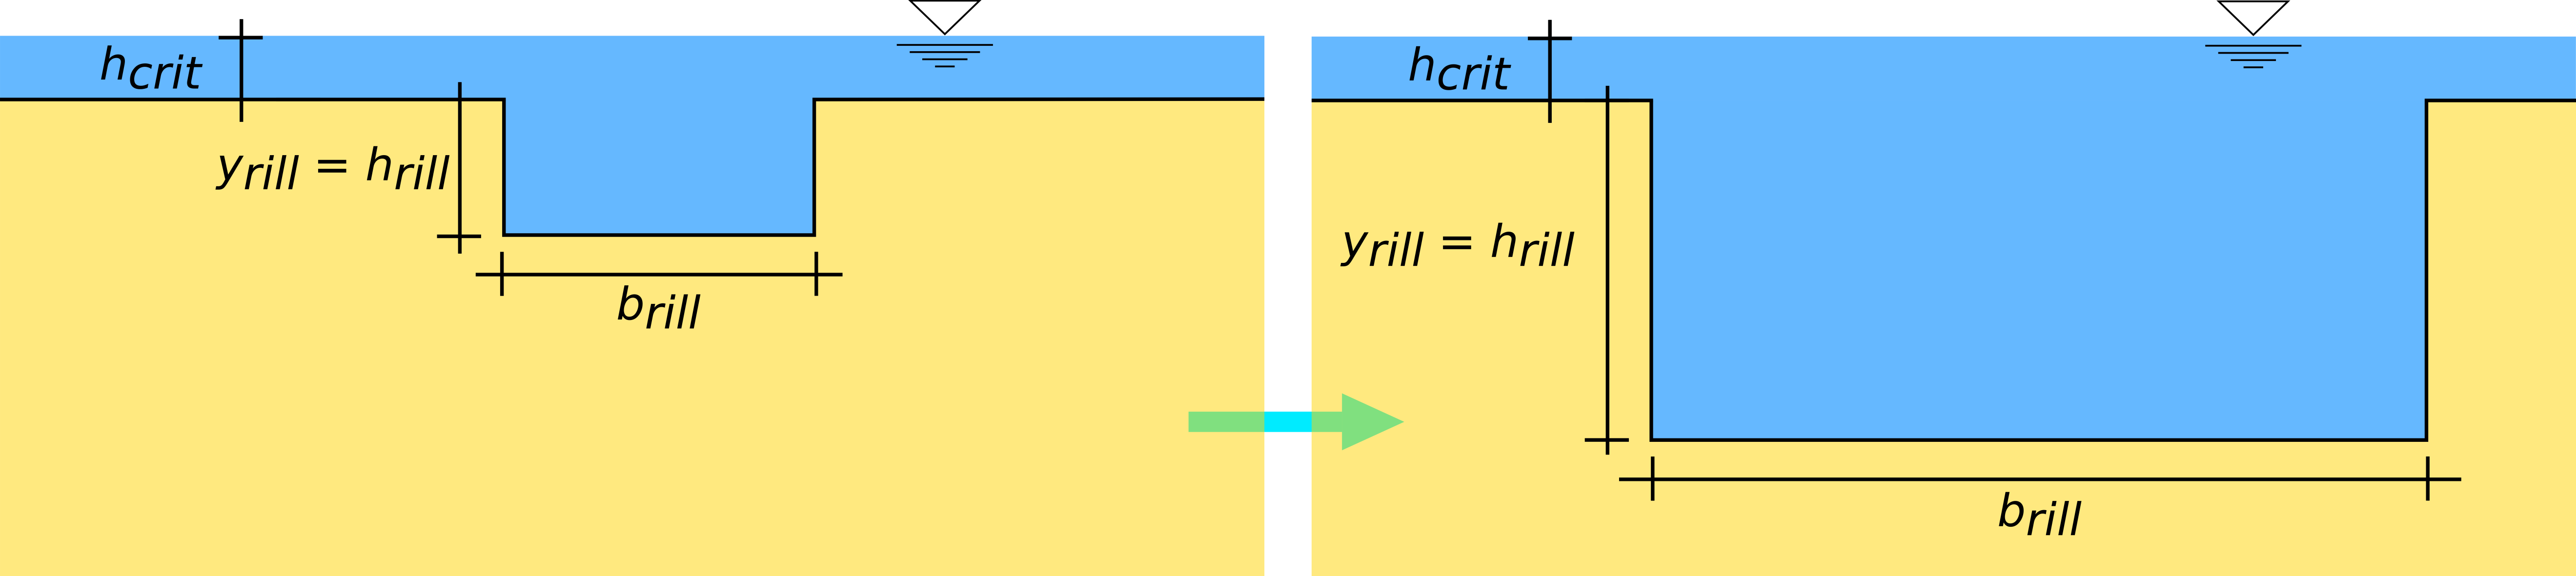
\includegraphics[width=1\linewidth]{./img/rill_schema_plneni.png}
      \caption{Příčný průřez rýhou, která se plní}
      \label{fig:rill_plneni}
    \end{subfigure}
    \begin{subfigure}[b]{1.\linewidth}
      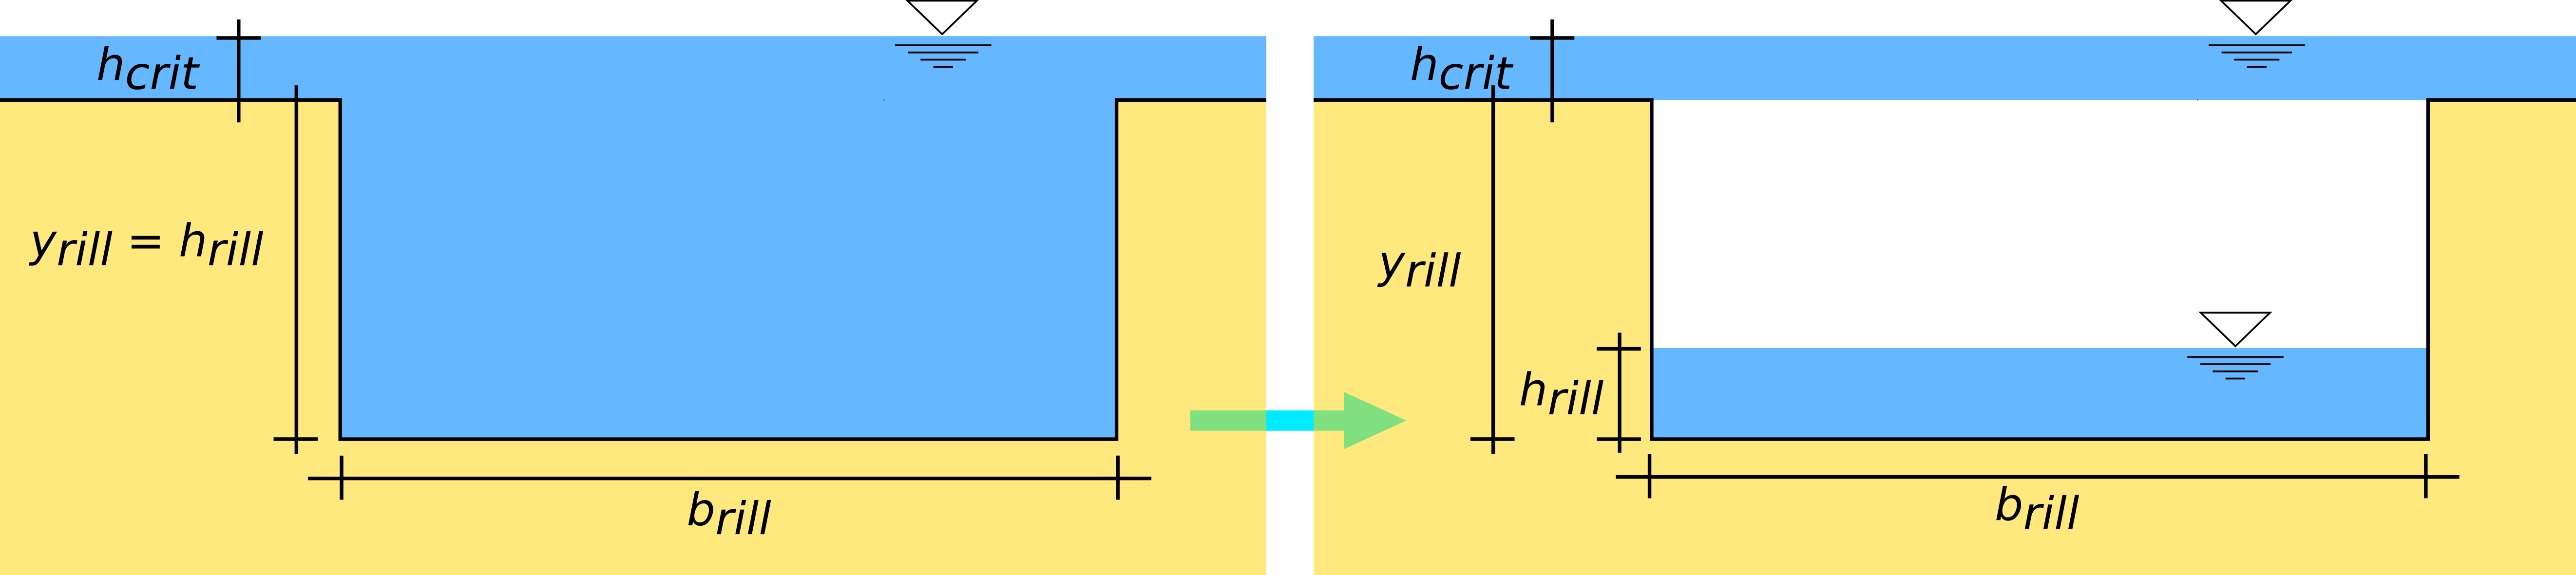
\includegraphics[width=1\linewidth]{./img/rill_schema_prazdneni.png}
      \caption{Příčný průřez rýhou, která se prázdní}
      \label{fig:rill_prazdneni}
    \end{subfigure}
    \caption{Příčný řez rýhou, která je v modelu \smod reprezentována obdélníkem.  Při plnění (zvětšování) rýhy roste výška hladiny vody v rýze s výškou rýhy  v poměru \acs{rratio} k šířce rýhy~(obrázek~\ref{fig:rill_plneni}).  Při prázdnění rýhy se tvar rýhy nemění, dochází pouze ke změně výšky vodní hladiny v rýze (nalevo) (obrázek~\ref{fig:rill_prazdneni}).}
    \label{fig:rill_schema}
  \end{figure}
% 
%   

  
\end{enumerate}


% Pro výpočet průtoku v rýze \acs{qrill} je pak možné využít Chézyho rovnici v manningově tvaru:.

  Výška odtoku (resp. vtoku) z rýhy je vypočtena podle vzorce
  $$
    \acs{oinrill} (resp.\ \acs{ooutrill}) = \acs{dT}\frac{\acs{qrill}}{\acs{brill}\acs{lrill}},
  $$
  \begin{tabular}{rrl}
    kde \jj{lrill}{.}
  \end{tabular}

\subsection{Celková bilance}
Pokud dojde k vzniku rýh, je rovnice celkové bilance~(\ref{eq:bilancnirce}) rozšířena o členy vyjadřující soustředěný rýhový odtok a přítok z rýh sousedních buněk takto

\begin{equation} 
\acs{hsur}_{i,t} = \acs{hsur}_{i,t-1} + \acs{dT}\left(\acs{es}_{i,t-1} + \sum_j^m \acs{oin}_{j,t-1} - \acs{inf}_{i,t-1} - \acs{oout}_{i,t-1}  + \sum_k^n \acs{oinrill}_{k,t-1} - \acs{ooutrill}_{i,t-1} \right),
\label{eq:bilancnircerill}
\end{equation}
  \begin{tabular}{rrl}
    kde \jj{oinrill}{\ a}
        \jj{ooutrill}{.}
        & $n$ & jsou buňky, odkud vtéká voda z rýh do buňky $i$.
  \end{tabular}\\
 Množství $n$ může být prázdná množina pokud není překročena kritická výška hladiny.





 
 
 
 
 
 
 
% Množství odtoku \acs{Orill} za \acs{dT} je pak možné stanovit podle vztahu:
% \begin{eqnarray}
% O_{rill_{i,t}} [m^{3}] = \Delta t q_{sur}
% \end{eqnarray}
% 
% Tvar bilanční rovnice \ref{bilancnirce} při zavedení odtoku v rýhách pak přechází na tvar:
% \begin{eqnarray}
%   H_{i,j,t} = H_{i,j,t-1} + ES_{i,j,t} + \sum\limits_{(i,j)\in M} O_{M_{t-1}} - O_{i,j,t} - I_{nf_{i,j,t}} \label{eq:bilancenew}
% \end{eqnarray}
% \begin{equation*}
%  M = \{ (k,l) | i-1 \leq k \leq i+1 ; j-1 \leq l \leq j+1 \}
% \end{equation*}



% \textit{kde $ O_{M} $ obecně znamená jak přítok plošný, tak soustředěný v rýhách, $ O $ celkový odtok, který se podle konkrétního stavu dělí na plošný a soustředěný}




\pozn{
\subsection{Poznámka nebo to dát do diskuse k článku} 
\begin{itemize}
\item Výsledný tvar blíží Maningově rovnici
\begin{eqnarray}
Q =\frac A {1}{n} R_{h}^{2/3} S^{1/2}
\end{eqnarray}
\item Přesněji pro tvar této rovnice pro plošný odtok, kdy se předpokládá proudění vody  o malé hloubce a tvar koryta je nahrazen jeho šířkou. Rovnice má pak tvar:
\begin{eqnarray}
Q =\frac {1}{n} h^{2/3} S^{1/2}
\end{eqnarray}
\item Že může být jiná rce infiltrace.
\item tvar rýhy - výzkum funkce?
\item jen jedna přímá rýha
\end{itemize}
}


%newb = math.sqrt(V/(rillRatio*l)) #KAvka, tohl eje divně
\section{Odtok hydrografickou sítí} \label{sec:tokyodtok}


Hlavní použití modelu \smod spočívá především v navrhování půdo ochranných opatření v ploše povodí. Cílem je simulovat a navrhovat odtoky i v dočasné hydrografické síti, která je tvořena přirozeným nebo častěji umělým přerušením přirozené odtokové dráhy. Nejčastěji se jedná o příkopy či průlehy, které mají odváděcí a protierozní funkci. 
Všechny prvky (síť vodních toků, příkopy, průlehy, atp.) jsou zadávány v rámci jedné liniové vektorové vrstvy, kde jsou úseky hydrografické sítě reprezentovány jednotlivými liniemi. 

Na rozdíl od výpočtu  povrchového odtoku, který je prováděn v rastru buněk, se  výpočet řeší v hydrografické síti po jednotlivých úsecích po skončení výpočtu povrchového odtoku. Jeden úsek hydrografické sítě zpravidla leží na několika buňkách rastru. Při výpočtu povrchového odtoku se do tohoto úseku započítá přítok ze všech buněk, které vtékají do buněk pod daným úsekem. Poté co výpočet povrchového odtoku skončí, provede se ve stejném časovém kroku výpočet odtoků a vtoků mezi jednotlivými úseky a spočítá se nová výška hladiny ve všech úsecích najednou. Princip propojení jednotlivých úseků je popsán v kapitole~\ref{sec:tokyodtok2}

Proudění v úsecích je řešeno Manningovou rovnicí ve tvaru:

\begin{equation}
    \acs{qstream} = \acs{A} \frac{1}{\acs{n}} \acs{Rstream}^{2/3} \acs{I}^{1/2}  ,
    \label{eq:qtok}
\end{equation}

% 
\begin{tabular}{rrl}
   kde \jj{qstream}{,}
       \jj{A}{,}
       \jj{n}{\ a}
       \jj{Rstream}{.}
\end{tabular}
  

Pro vlastní výpočet je třeba zadat typ a příčný profil daného úseku. Délka úseku a jeho sklon jsou převzaty z liniové vrstvy a z digitálního modelu terénu. Protože je model určen pro malá povodí, jsou v modelu předpokládány pouze základní tvary příčných profilů (trojúhelník, obdélník, lichoběžník, parabola). Vzorce pro výpočet odtoku různými geometriemi příčných profilů jsou ukázány  v tabulce~\ref{fig:tvary_koryt} v příloze \ref{sec:priloha}. Model \smod je schopen řešit odtok liniovými prvky, které se zapojí do odtoku až při tvorbě povrchového odtoku, i~odtok vodními toky se základním odtokem. Princip zadávání geometrie úseků hydrografické sítě je popsán v kapitole~\ref{sec:vodnitoky} v části~\ref{cast:2} tohoto manuálu. 
  
Objem vody, který teče mezi jednotlivými úseky hydrografické sítě je určen jako
$$
  V_{stream,out} = \acs{dT}\acs{qstream}.
$$



% \pozn{a dát semka asi i nějaké  obrázky, jak to funguje. Je to v nějaké DP tuším (to najdu PK)}


\begin{figure}[b!]
  \centering
  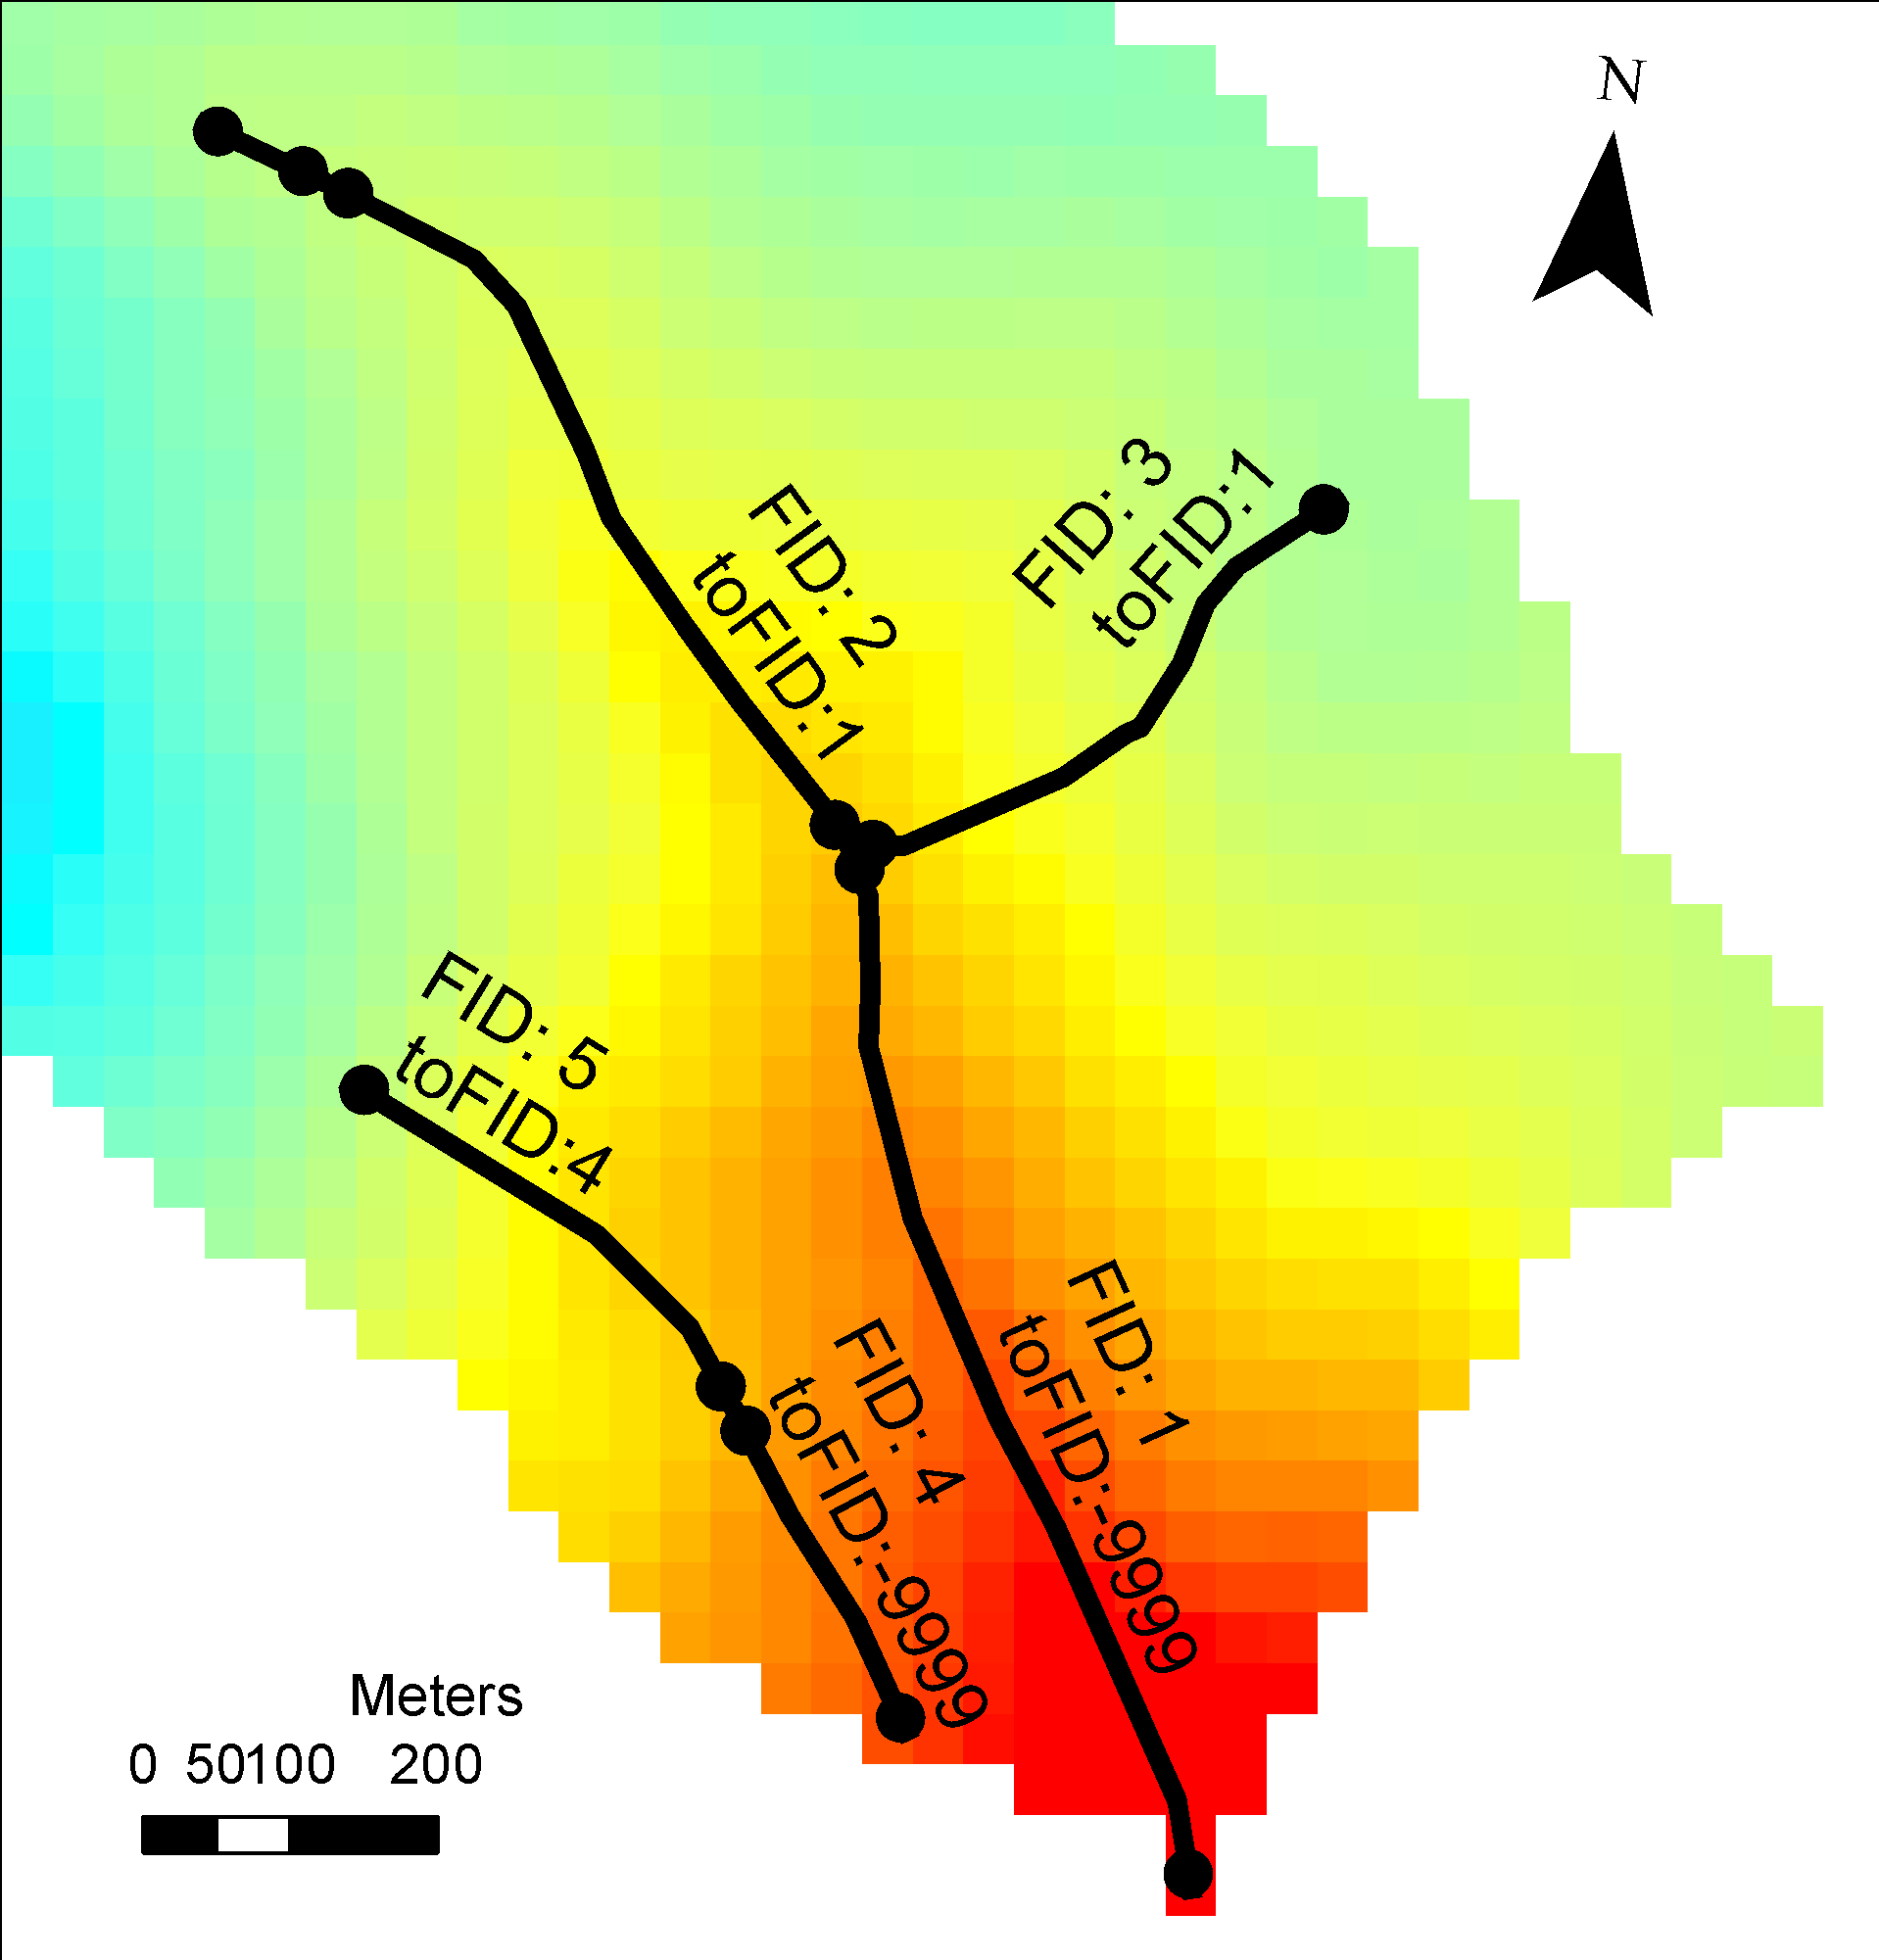
\includegraphics[width=0.5\textwidth]{./img/mapalinie.png}
  \caption{Hydrografická síť s označením {\tt FID} (id linie) a {\tt toFID} (id následující linie při odtoku). Podkladová vrstva je digitální model terénu. {\tt toFID} = -9999 označuje  odtok přes okraj výpočetní oblasti.}
  \label{fig:mapalinie}
\end{figure}

\subsection{Propojení úseků hydrografické sítě} \label{sec:tokyodtok2}


Na obrázku \ref{fig:mapalinie}, jsou ukázány úseky na podkladové vrstvě digitálního modelu terénu. Každý úsek má označení {\tt FID}. Při přípravě dat dostane každý úsek atribut {\tt toFID}, který udává, s jakými úseky je daný úsek propojen ve směru odtoku. {\tt toFID} = -9999 značí odtok přes okraj výpočetní oblasti. 



Pří přípravě dat je opraven směr úseku podle digitálního modelu terénu. Pokud má úsek oba koncové body v stejné výšce (sklon úseku je nulový), program se ukončí s chybovým hlášením: {\tt ZeroSlopeError: 'Reach FID:1 has zero slope.'}. Chybové hlášení označí problematický úsek (v této ukázce úsek s {\tt  FID = 1}) a uživatel musí daný úsek opravit ve vstupních datech tak, aby měl nenulový sklon (aby koncové body úseku nebyly ve stejné výšce).  









% \pozn{ Tímto způsobem jsou zadány tvary prvků, které se v řešené lokalitě vyskytují.
% \textbf{sem dát obrázek těch profilů}}


% \pozn{\textbf{doplnit text jak probíhá vlastní výpočet} - tzn jak na sebe navazují jednotlivé úseky . a dát semka asi i nějaké  obrázky, jak to funguje. Je to v nějaké DP tuším (to najdu PK)}


